%%%%%%%%%%%%%%%%%%%%%%%%%%%%
%%%%%%    PREFACE     %%%%%% 
%%%%%%%%%%%%%%%%%%%%%%%%%%%%
\documentclass[11pt]{article}
\usepackage[letterpaper, margin=1in]{geometry}

% load packages
\usepackage{natbib}         % cite references
\usepackage{multibib}
\newcites{rev}{References}  % citep --> citeprev; citet --> citetrev
\usepackage[utf8]{inputenc}       % noindent
\usepackage[dvipsnames]{xcolor}   % use colors
\usepackage{authblk}              % author names
\usepackage{ragged2e}       % align text
\usepackage{booktabs}       % use tables
\usepackage{multirow}       % use multirow
\usepackage{graphicx}       % using figures
\usepackage{caption}        % set no caption numbers for figures
\usepackage{amsthm}         % use mathematics
\usepackage{soul}           % wrapped underline 

% set font
\usepackage[sfdefault]{ClearSans}
\usepackage[T1]{fontenc}

\usepackage{xr-hyper}        % use cross references
\externaldocument{materials} % link the external
\externaldocument{03-revise} % link the external 
\usepackage{hyperref}        % use hyperlinks
\hypersetup{colorlinks=true, citecolor=black, linkcolor=black, urlcolor=blue}

% set the paper as noindent
\setlength\parindent{0pt}

% initialize counters for reviewer and comments 
\newcounter{reviewer}
\setcounter{reviewer}{0}
\newcounter{point}[reviewer]
\setcounter{point}{0}

% set the format of responses
%% point
\renewcommand{\thepoint}{Comment\,\thereviewer.\arabic{point}:} 
\newcommand{\point}[1]{\refstepcounter{point} \bigskip \noindent {\fontseries{b}\selectfont \thepoint} #1 \par}
%% response
\newcommand{\sect}[1]{{\bigskip \bigskip \textbf{\noindent #1} }} % for section 
\newcommand{\reply}[1]{\bigskip \textcolor{blue}{\noindent \textbf {Reply:} #1}}
\newcommand{\nextreply}[1]{\bigskip \textcolor{blue}{\noindent #1}}
\newcommand{\marked}[1]{\bigskip \textit{\textcolor{blue}{\noindent #1}}}
\newcommand{\revised}[3][2]{\bigskip \textcolor{magenta}{\noindent \textbf{Line #2:} #3}}
%% reviewer headings
\newcommand{\editorsection}{\newpage \section*{Editor} \hrule}
\newcommand{\reviewersection}{\newpage \stepcounter{reviewer} \section*{Reviewer \thereviewer} \hrule}
% to-do command
\newcommand\myTodo[1]{\textcolor{red}{! #1}}

%%%%%%%%%%%%%%%%%%%%%%%%%%%%%%%%%%%%%%%%%%%%%%%%
%%%%%%%%%%%%    BEGIN BEGIN BEGIN   %%%%%%%%%%%%
%%%%%%%%%%%%%%%%%%%%%%%%%%%%%%%%%%%%%%%%%%%%%%%%

% title page
\title{\raggedright {Response to Editors' and Reviewers' Comments:}
{\textbf{Significant regime shifts in historical water yield in the Upper Brahmaputra River basin}}}

\begin{document}
\date{}
\author{}
\maketitle
% Vim: i: inerst; Ctrl + C: exit 
%%%%%%%%%%%%%%%%%%%%%%%%%%%%%%%%%%%%%%%%%%
% general comments 
%%%%%%%%%%%%%%%%%%%%%%%%%%%%%%%%%%%%%%%%%%
Dear Dr. Giulia Zuecco, \\

Thanks for the comments and suggestions from you and three reviewers in the past several rounds of review. Now, we addressed some technological corrections, mainly including (1) careful English checks, (2) updated figures, and (3) a repository for data, Python codes and LaTex scripts. We hope that the revised manuscript can meet the standards of the Journal \textit{Hydrology and Earth System Sciences}. \\

In addition, we decided to use a much more clear, tightly constructed title \textbf{"Significant regime shifts in historical water yield in the Upper Brahmaputra River basin"}. We believe that it can improve the chances of the manuscript being discovered by relevant researchers and the public. \\

Below we provide a point-by-point response to the comments and concerns raised by the editor and reviewers. All modifications in the manuscript have been marked. \\

Sincerely

\begin{flushleft}

Hao Li (on behalf of all coauthors)  \\
PhD candidate, \url{Hao.liwork@ugent.be} \\
Hydro-Climate Extremes Lab, Ghent University \\
Nov 12, 2022 \\

\includegraphics[width=.15\textwidth]{02-figures/signature.png} \par
\end{flushleft}

%%%%%%%%%%%%%%%%%%%%%%%%%%%%%%%%%%%%%%%%%%
\editorsection
%%%%%%%%%%%%%%%%%%%%%%%%%%%%%%%%%%%%%%%%%%

%%%%%%%%%%%%%%%%%%%%%%%%%%%%%%%%%
\point{Thank you for submitting a revised version of the manuscript. As you can see, the first reviewer appreciated the revised manuscript, but he noticed that the Python scripts cannot be accessed because a password is required.}
\reply{We are so sorry that we did not double check that. We have created a Git repository that is connected Zenodo.}

%%%%%%%%%%%%%%%%%%%%%%%%%%%%%%%%%%%%%
\point{A careful revision of the English by a native speaker is needed due to unclear sentences, typos, and repeated words (e.g., lines 24-26 in the manuscript without track changes, lines 246-247, lines 266-268 etc.).}
\reply{Thank you very much for your suggestion. We have revised the whole manuscript and carefully proofread the manuscript to minimize typographical, grammatical, and bibliographical errors. A native English speaker was also invited to check the language. We believe that the language is now acceptable for the review process.}

\nextreply{Relevant revisions are shown:}

\revised{22--25}{Therefore, WY changes over this region significantly affect water availability, terrestrial and aquatic ecosystems which are vital for sustaining the livelihoods of approximately two billion people \citeprev{immerzeel2010climate}. Despite some in-situ observations and estimates from state-of-the-art remote sensing \citeprev{wang2021tp}, total river runoff has never been reliably assessed in this region, and its response to global warming remains unclear.}

\revised{245--248}{However, in some mountainous basins, human activities such as urbanization, dam regulation and irrigation may consume a significant portion of water resources or induce changes in seasonal runoff patterns. Therefore, it is necessary to account for anthropogenic impacts when assessing river flow changes via the statistical models in these regions, in addition to the factors considered in this study.}

\revised{267--270}{However, LAI ignores the vegetation's physiological process \citeprev{fang2019overview}. \citetrev{hu2022decoupling} have indicated that LAI can cope with hydro-climatic fluctuations in arid environments, but the tradeoff between ecosystem structure (LAI) and physiology (photosynthesis per unit leaf area) is stronger in humid climates. Thus, using LAI products in energy-limited regions may result in some biased assessments of vegetation effects on water yield.}

%%%%%%%%%%%%%%%%%%%%%%%%
\point{Fig. 2a: Please add the legend for the dots.} 
\reply{Thanks for your comment. We have updated Figure 2a with a clearer illustration.}

%%%%%%%%%%%%%%%%%%%%%%%
\point{Please check that all acronyms are explained and described correctly in the manuscript.}
\reply{Thanks. We have checked the acronyms in the manuscript. Now, all of them have been defined in a clear way.}

%%%%%%%%%%%%%%%%%%%%%%%%
\point{Fig. 4a: Please explain in the caption what $\Delta$R means.}
\reply{Thanks for your comment. We deleted $\Delta$R in the figure. Instead, we added detailed descriptions in the caption.}

\begin{figure*}[ht]
    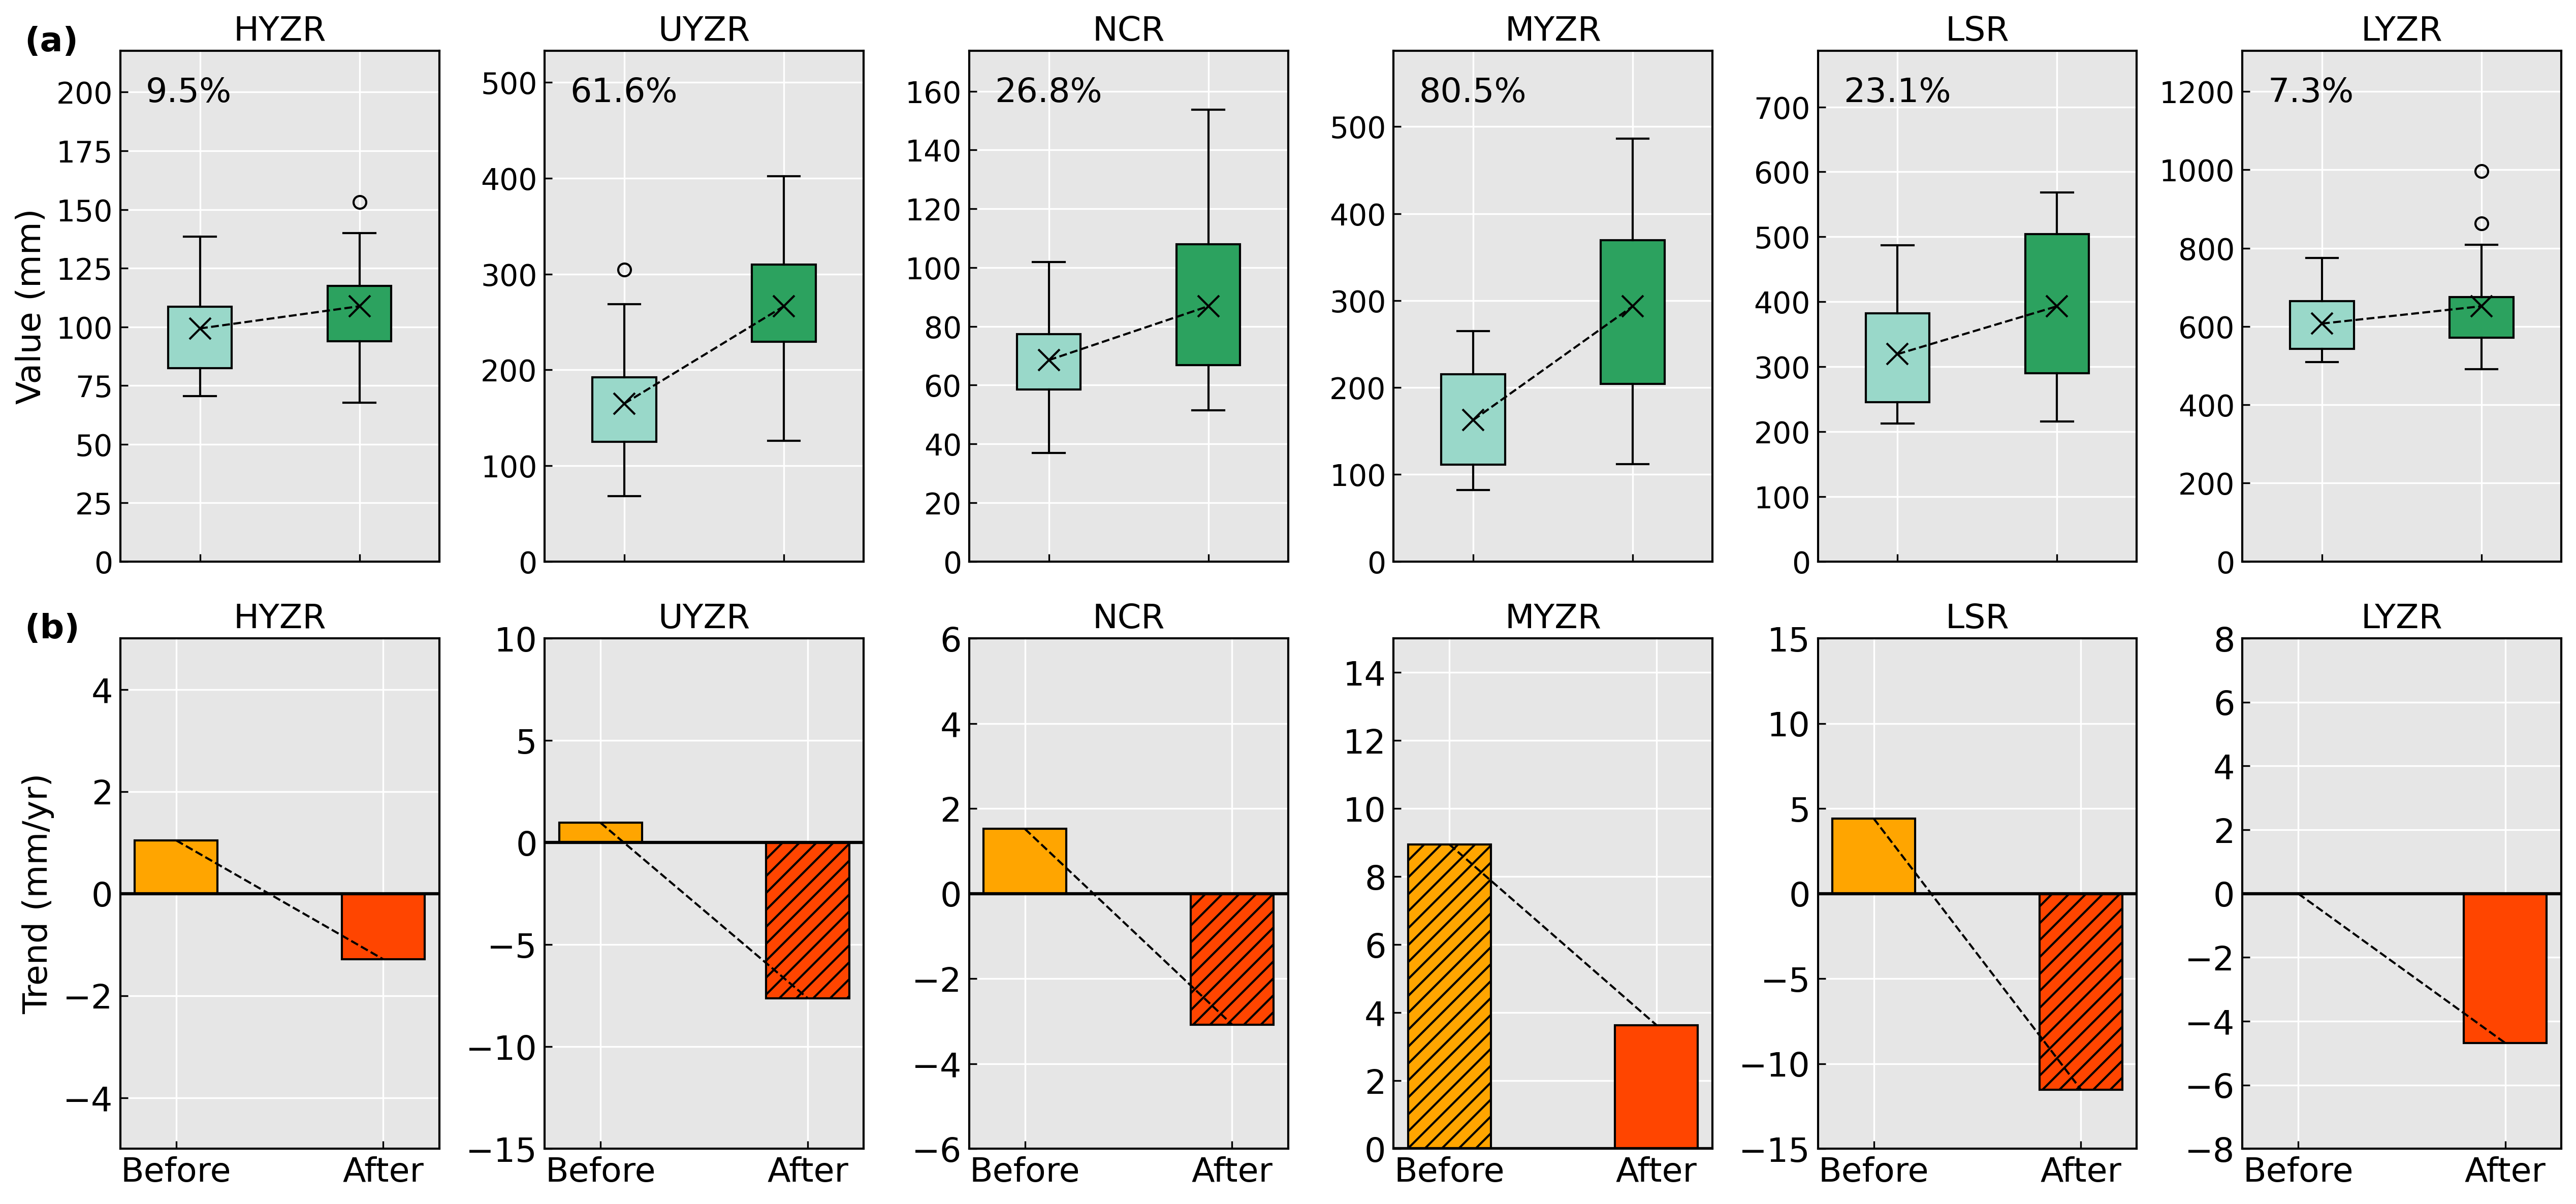
\includegraphics[width=\textwidth]{02-figures/magnitude_and_direction.png}
    \captionsetup{labelformat=empty}
    \caption
    {Figure 4. Water yield regime shifts in the entire UBR basin. (a) Magnitude of water yield changes. The black "x" signal shows the mean of water yield, \textbf{and the relative change is labeled in number (\%) in each boxplot}. (b) Direction of water yield changes. The black hatching represents the statistically significant trend (p < 0.05). The color of boxes represents before (light color) and after (dark color) Tp period.}
    \label{fig:magnitude-direction}
\end{figure*}

%%%%%%%%%%%%%%%%%%%%%%%
\point{Fig. S1, S2, S5, S7 and S9: Please increase the size of the labels (some are too small and it is difficult to read them).}
\reply{Thanks for your reminder. We have updated these figures in the supplementary.}

\bibliographystylerev{copernicus}
\bibliographyrev{reference.bib}


%%%%%%%%%%%%%%%%%%%%%%%%%%%%%%%%%%%%%%%%%%
\reviewersection % reviewer 01
%%%%%%%%%%%%%%%%%%%%%%%%%%%%%%%%%%%%%%%%%%
\sect{Technical corrections}

\point{Thank you again for addressing my comments. I think the paper is now in a state that can be published. There is just one problem that I cannot access the repository, as I asks me for a password, which I do not have. I would be better to just publish it as a public repository on Github, while also making citable with Zenodo (https://zenodo.org). This would make sure that a fixed version of the Code is assigned to the paper.}
\reply{Thank you very much for your comments and suggestions in past several rounds of review. We have created a Git repository that is connected by Zenodo.}

\nextreply{Also, we decided to use the new title \textbf{"Significant regime shifts in historical water yield in the Upper Brahmaputra River basin"}. We believe that it is much more clear, tightly constructed and also can improve the chances of the manuscript being discovered by relevant researchers and the public. I am very glad to hear your opinions.}

\bibliographystyle{copernicus}

\end{document}
